% !TeX root = ../thesis.tex

\chapter{Data}
\label{app:Data}

\begin{figure}[!h]
	\centering
	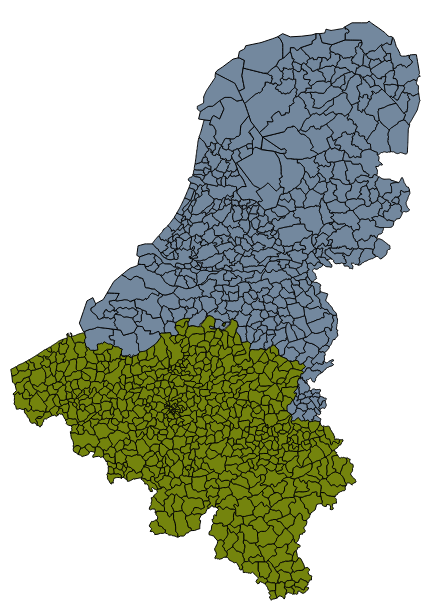
\includegraphics[width=0.5\linewidth]{figs/Municipalities.png}
	\caption{Dataset of municipalities in the Netherlands and Belgium in 2015 (from Dutch cadaster and GADM.org)}
	\label{fig:municipalities}
\end{figure}

\begin{figure}[!h]
	\centering
	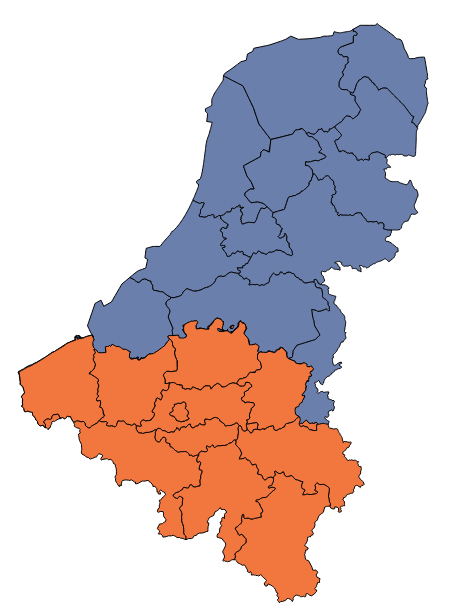
\includegraphics[width=0.5\linewidth]{figs/Provinces.png}
	\caption{Dataset of provinces in the Netherlands and Belgium in 2015 (from Dutch cadaster and GADM.org)}
	\label{fig:provinces}
\end{figure}

\begin{figure}[!h]
	\centering
	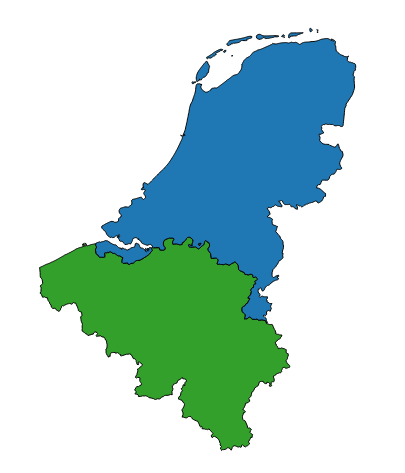
\includegraphics[width=0.5\linewidth]{figs/Countries.png}
	\caption{Dataset of the Netherlands and Belgium in 2015 (from GADM.org)}
	\label{fig:countries}
\end{figure}

\begin{figure}[!h]
	\centering
	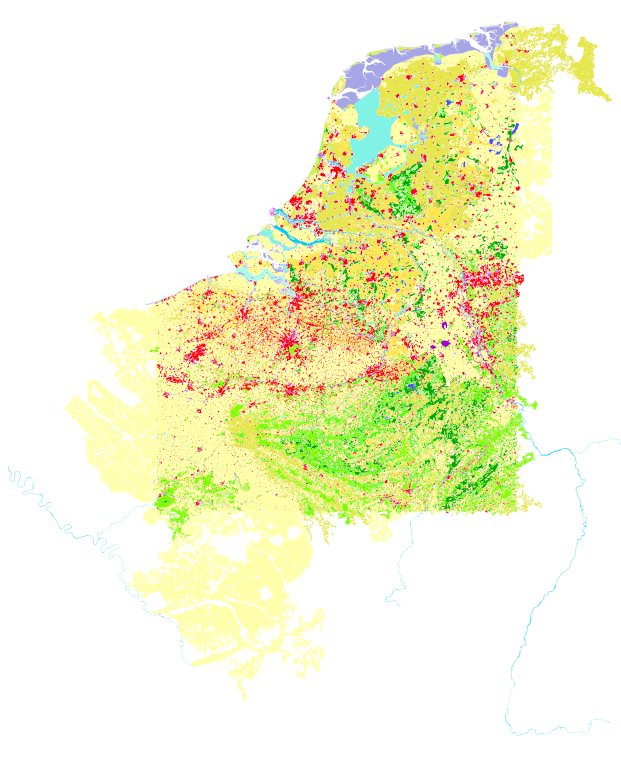
\includegraphics[width=1\linewidth]{figs/CORINE_NL_BE_color.PNG}
	\caption{Dataset of landcover in the Netherlands and Belgium in 2012 (from Copernicus  The European Earth Observation Programme)}
	\label{fig:CORINE}
\end{figure}

\begin{figure}[!h]
	\centering
	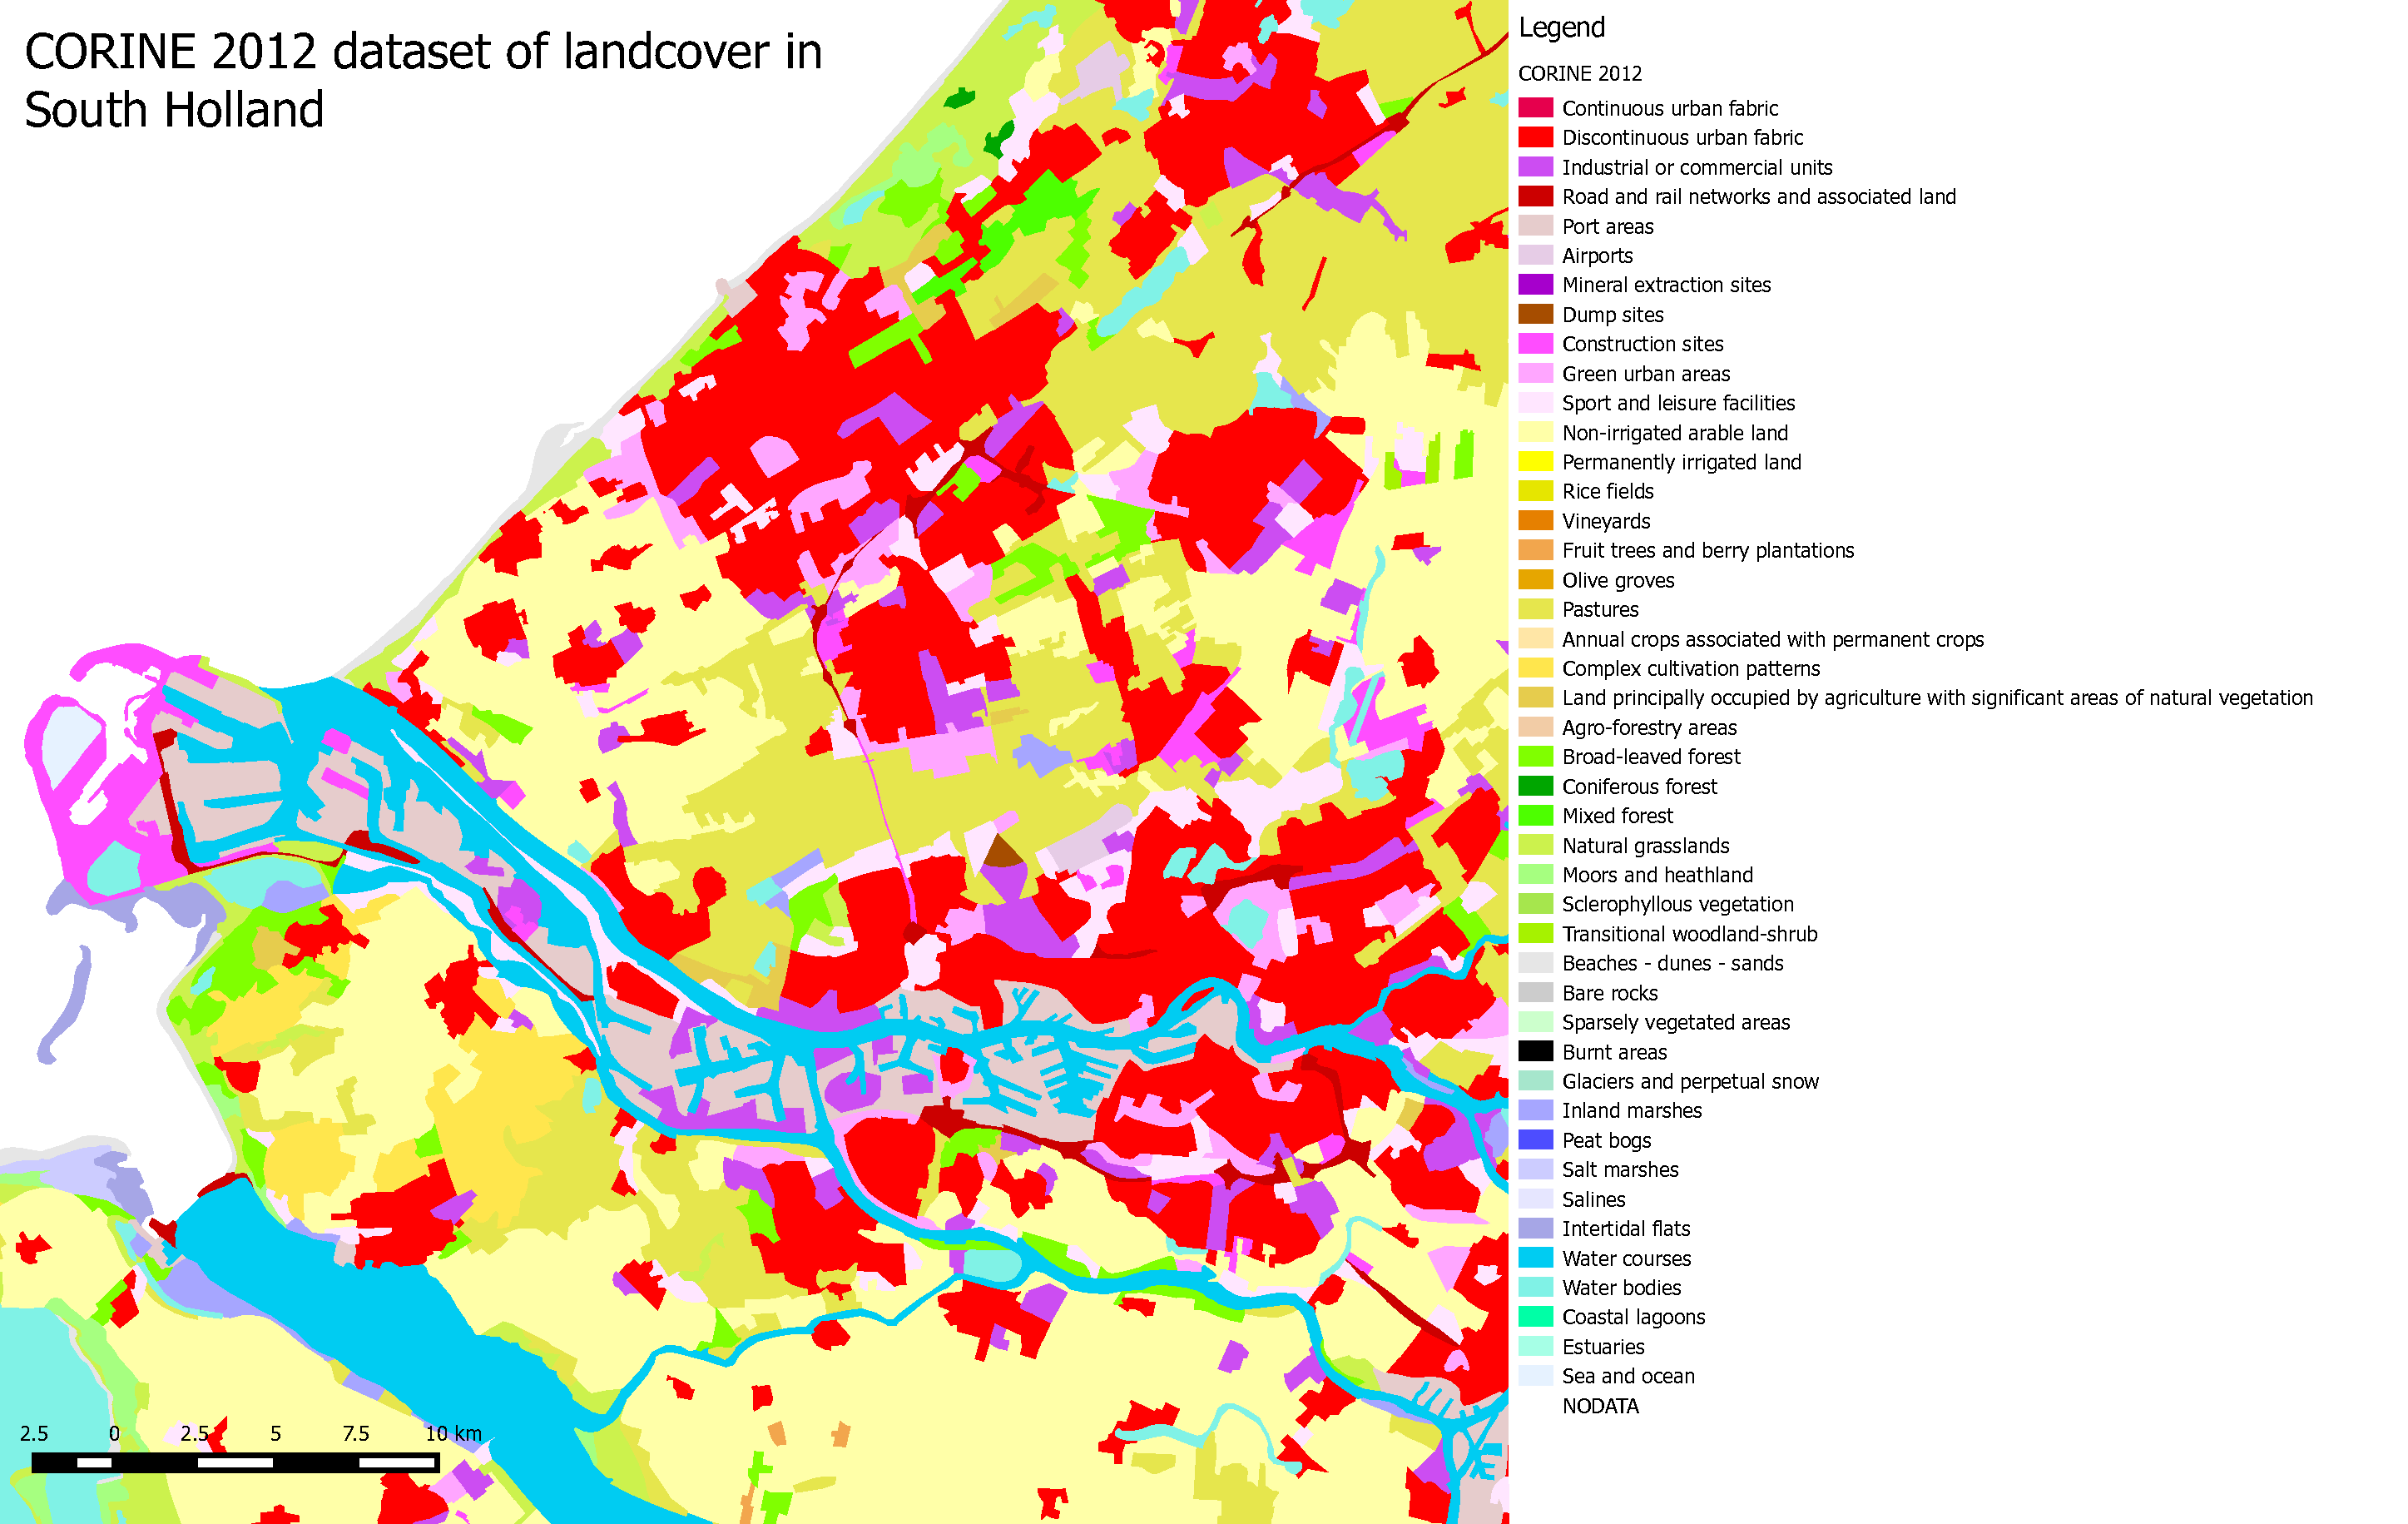
\includegraphics[width=1\linewidth]{figs/CORINE_NL_BE_color_zoom.PDF}
	\caption{Landcover of the province of South Holland (subsection of the dataset from Figure \ref{fig:CORINE})}
	\label{fig:CORINEZOOM}
\end{figure}

\begin{figure}[!h]
	\centering
	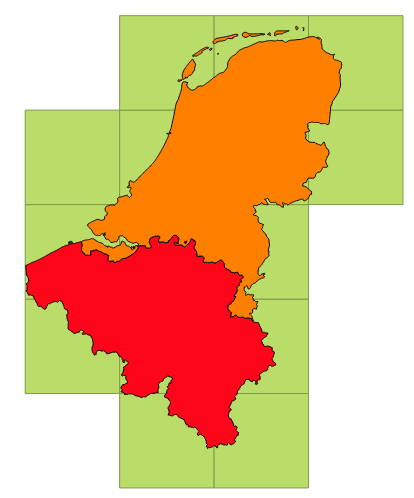
\includegraphics[width=0.7\linewidth]{figs/EEA100km.png}
	\caption{\ac{eea} reference grid cells with a resolution of 100km\textsuperscript{2} overlapping the Netherlands and Belgium}
	\label{fig:100KM}
\end{figure}

\begin{figure}[!h]
	\centering
	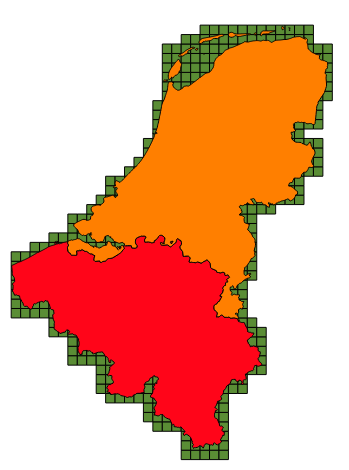
\includegraphics[width=0.7\linewidth]{figs/EEA10km.png}
	\caption{\ac{eea} reference grid cells with a resolution of 10km\textsuperscript{2} overlapping the Netherlands and Belgium}
	\label{fig:10KM}
\end{figure}

\begin{figure}[!h]
	\centering
	\includegraphics[width=0.6\linewidth]{figs/RIVMSensors.png}
	\caption{Webmap by the \ac{rivm} showing their air quality sensor network (\url{http://www.lml.rivm.nl/meetnet})}
	\label{fig:RIVMSensor}
\end{figure}

\begin{figure}[!h]
	\centering
	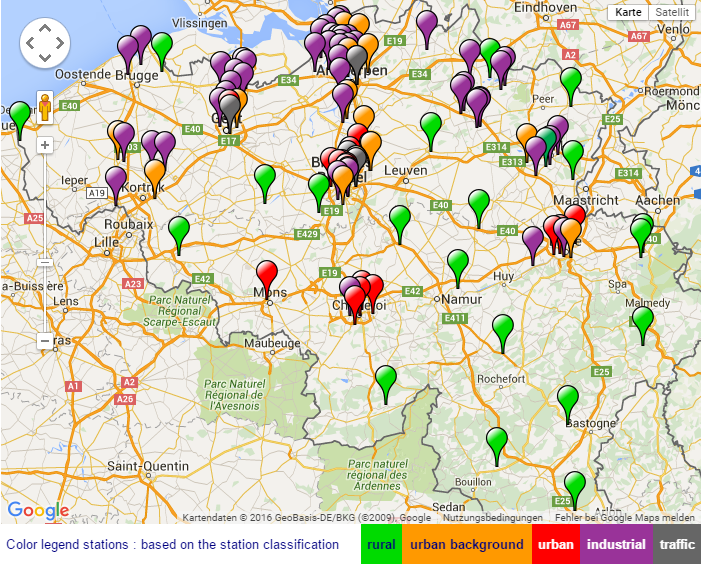
\includegraphics[width=0.6\linewidth]{figs/IRCELINESensors.png}
	\caption{Webmap by \ac{ircel} showing their air quality sensor network (\url{http://www.irceline.be/en/air-quality/measurements/monitoring-stations/})}
	\label{fig:IRCELINESensor}
\end{figure}

\begin{figure}[!h]
	\centering
	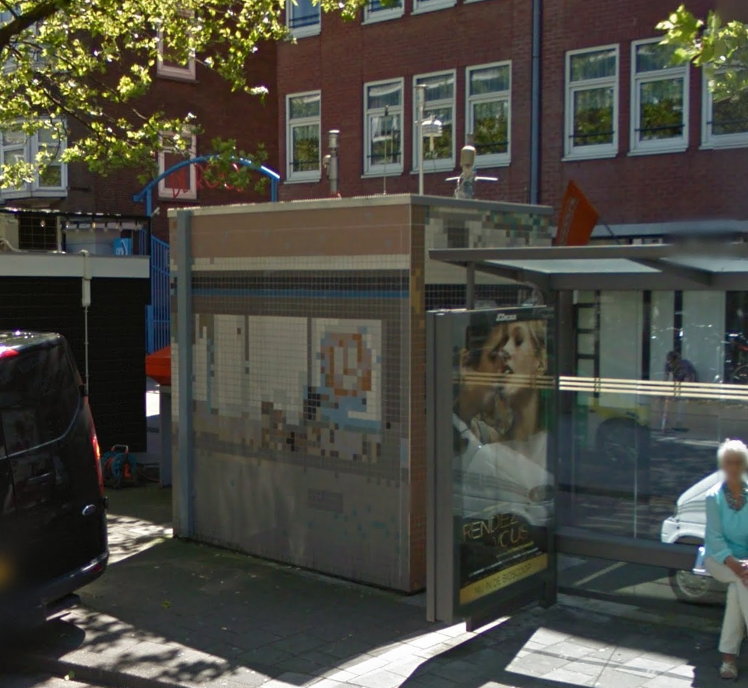
\includegraphics[width=1\linewidth]{figs/SensorAdam.png}
	\caption{Google Streetview image of \ac{rivm} sensor location in Amsterdam in 2015}
	\label{fig:Sensor}
\end{figure}
